\documentclass[12pt,a4paper]{article}
\usepackage{physics}
\usepackage{amssymb}
\usepackage{subcaption}
\usepackage{colortbl}
\usepackage{musicography}
\newcommand{\activity}{Activity 12 -- Feature Extraction}
\input{spp.dat}

\begin{document}

\title{\TitleFont \activity}
\author[ ]{\textbf{Kenneth V. Domingo} \\
2015--03116 \\
App Physics 186, 1\textsuperscript{st} Semester, A.Y. 2019--20}
\affil[ ]{\corremail{kvdomingo@up.edu.ph} }

\maketitle
\thispagestyle{titlestyle}

\section*{Results and Discussion}
\setcounter{section}{1}

For this activity \cite{soriano}, I obtained the Fruits-360 dataset from Kaggle \cite{kaggle} which contains thousands of labeled fruit images under the same lighting and capture settings but with varying angles. I took 50 samples each from the set of apples, oranges, and bananas.

\subsection{Feature extraction: $L^*a^*b^*$ color space}
I first imported the images into Python and converted them to $L^*a^*b^*$ color space. For each image, I extracted the mean values from the $a^*$ and $b^*$ channels. The $a^*$ channel represents a chromaticity from green to red, while the $b^*$ channel represents a chromaticity from blue to yellow.

\subsection{Feature extraction: eccentricity $e$}
Using the same images, I applied Otsu's method since the images contain only one fruit on a plain white background. Each fruit is then easily detected as a single large blob. I then used the \texttt{regionprops} function to extract the eccentricity property from each detected blob. An $e = 0$ corresponds to a perfect circle, while an $e = 1$ corresponds to a parabola. Values $0 < e < 1$ are ellipses.

\subsection{Discussion}
Figure \ref{fig:feature-space} shows the feature space of the selected dataset in $a^*$, $b^*$, and $e$. We can observe that all the classes show distinct clustering. The projections on each of the planes are shown in Fig. \ref{fig:projections}. The banana cluster shows a large variation in eccentricity but mostly resides in high-eccentricity space. This can be attributed to the various rotations of the banana images, but are still significantly elongated compared to the other fruit classes. Apples and oranges overlap in $a^*$ space (red and orange have very close chromaticities), but can be separated in the $b^*$--$e$ space (orange is closer to yellow than red is; apples are less rounded compared to oranges). If we needed to reduce the complexity, it is sufficient to choose between either $a^*$--$b^*$ or $b^*$--$e$ feature spaces, though the former appears to maximize the class separation.

\begin{figure}
	\centering
	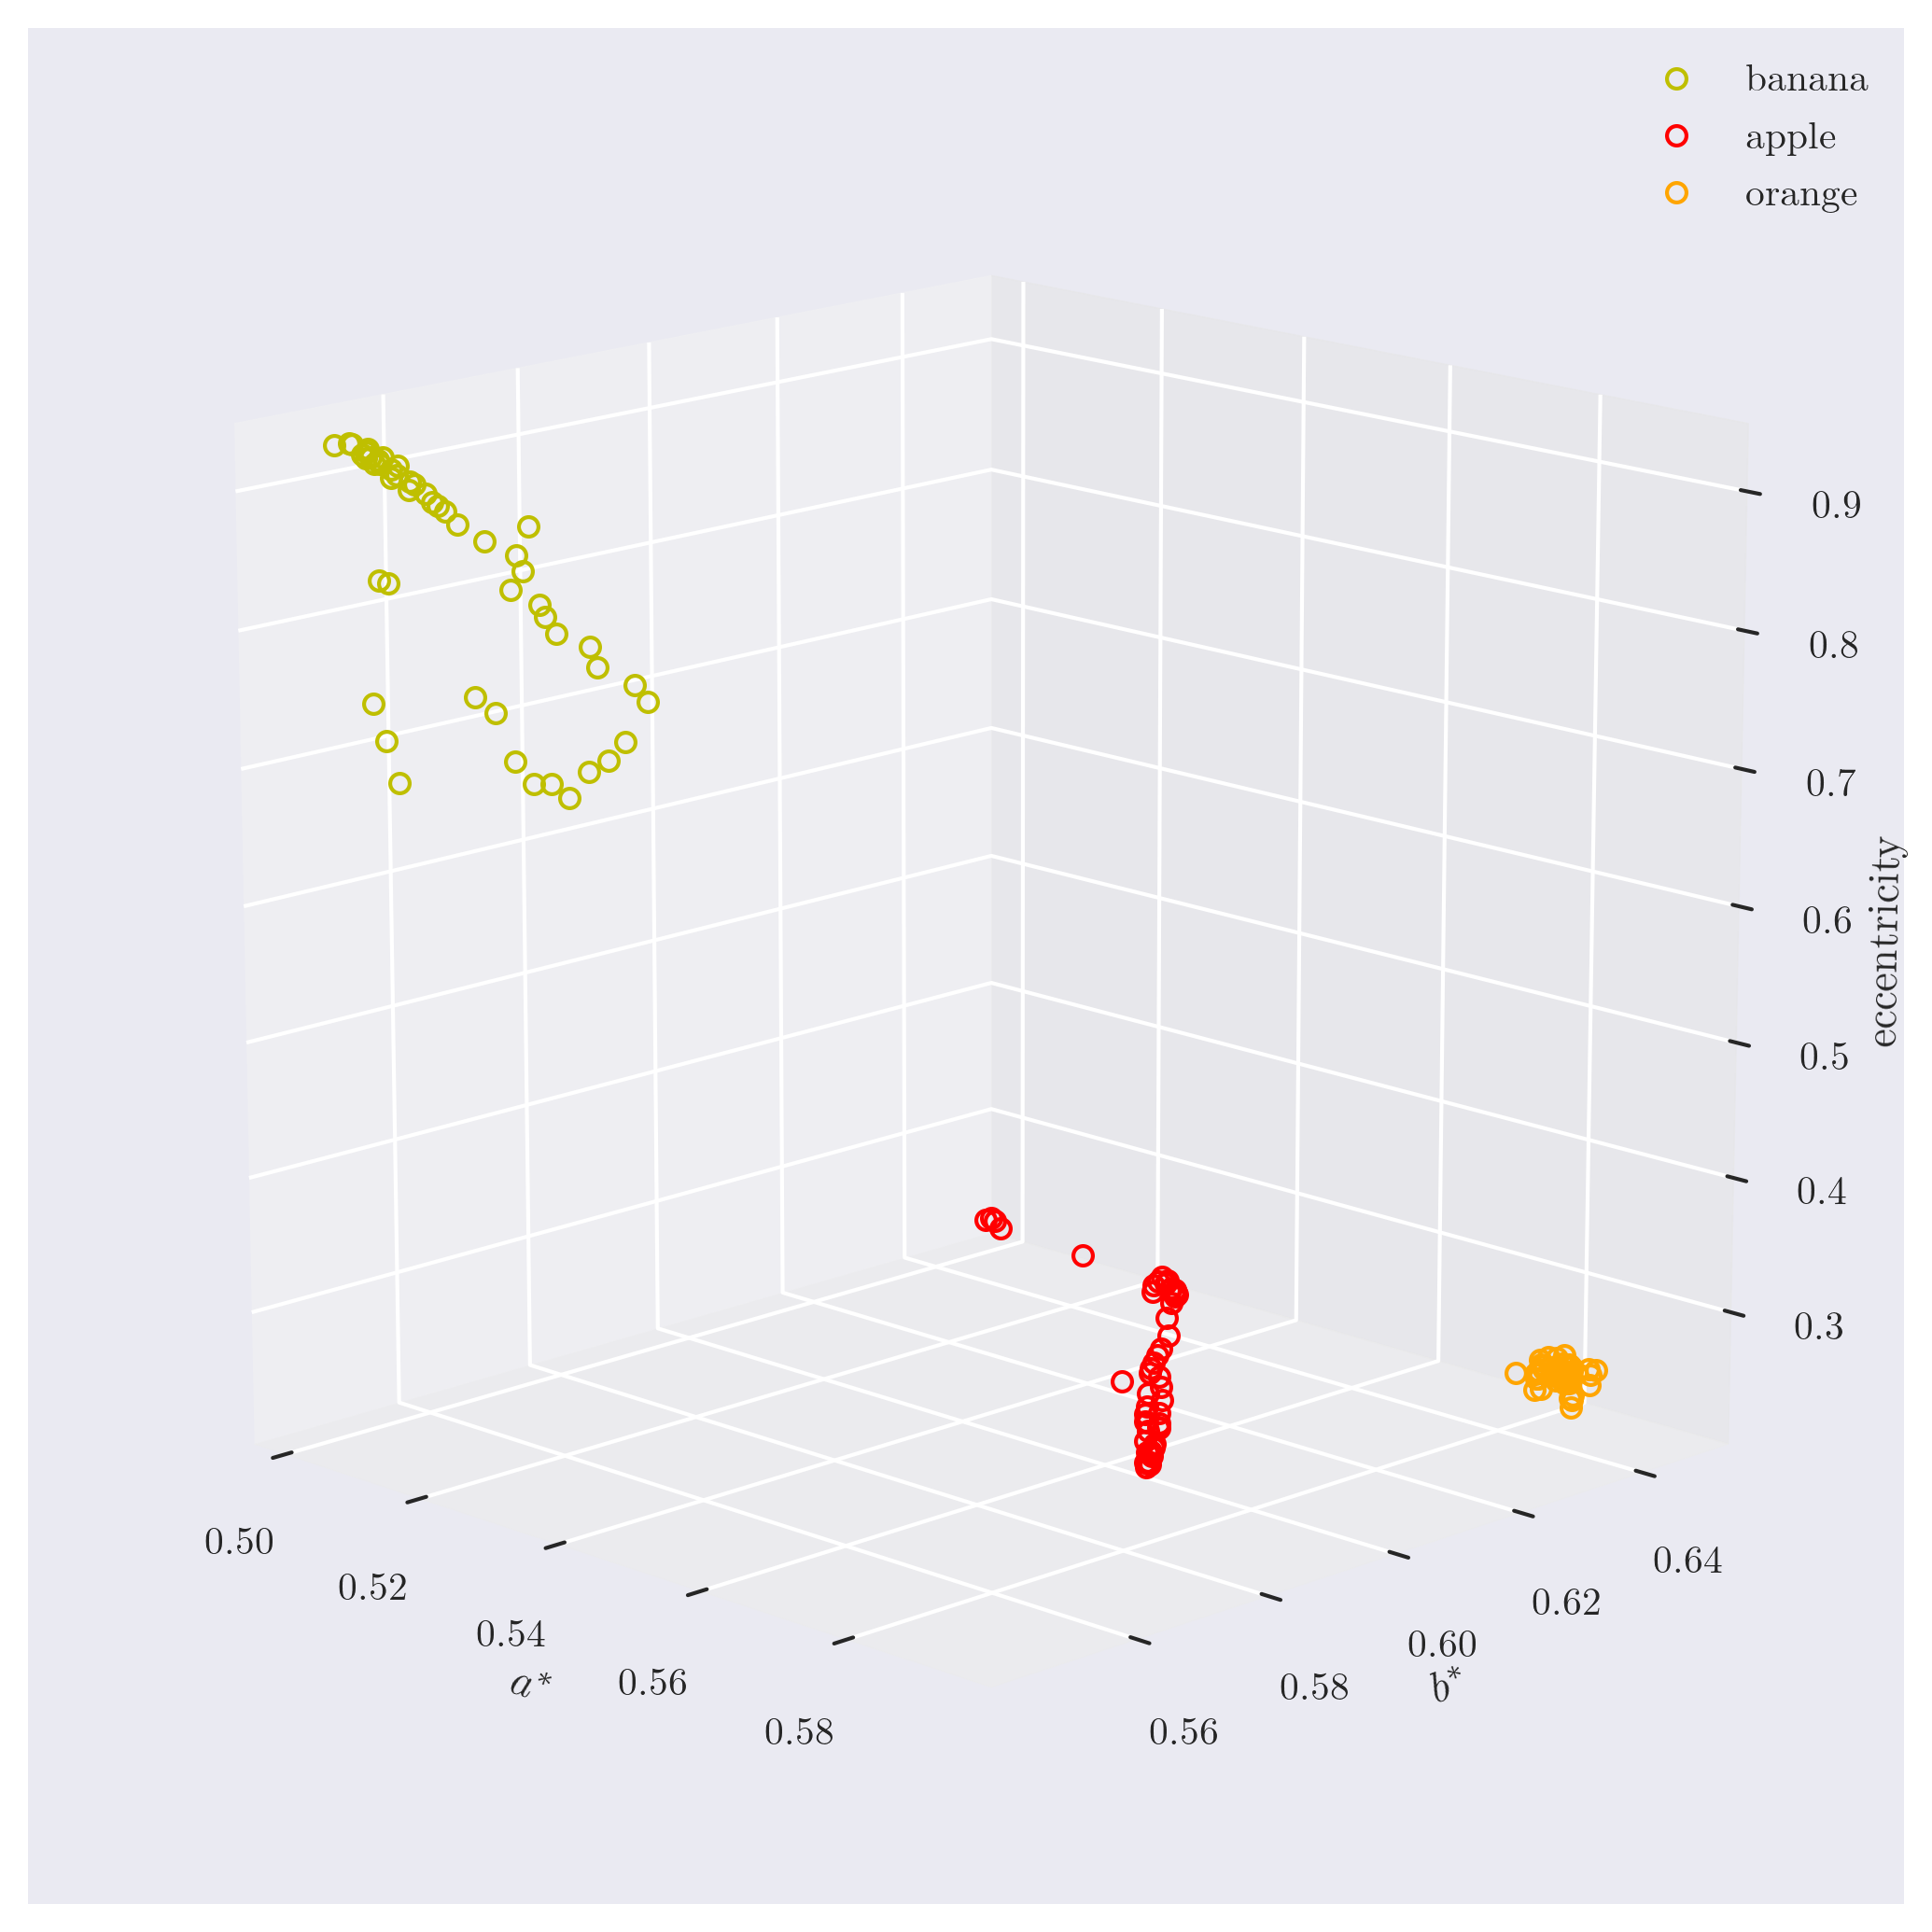
\includegraphics[width=0.75\textwidth]{feature_space.png}
	\caption{Feature space in $a^*$, $b^*$, and $e$ of apples, bananas, and oranges.}
	\label{fig:feature-space}
\end{figure}

\begin{figure}[htb]
	\centering
	\begin{subfigure}[h!]{0.3\textwidth}
		\centering
		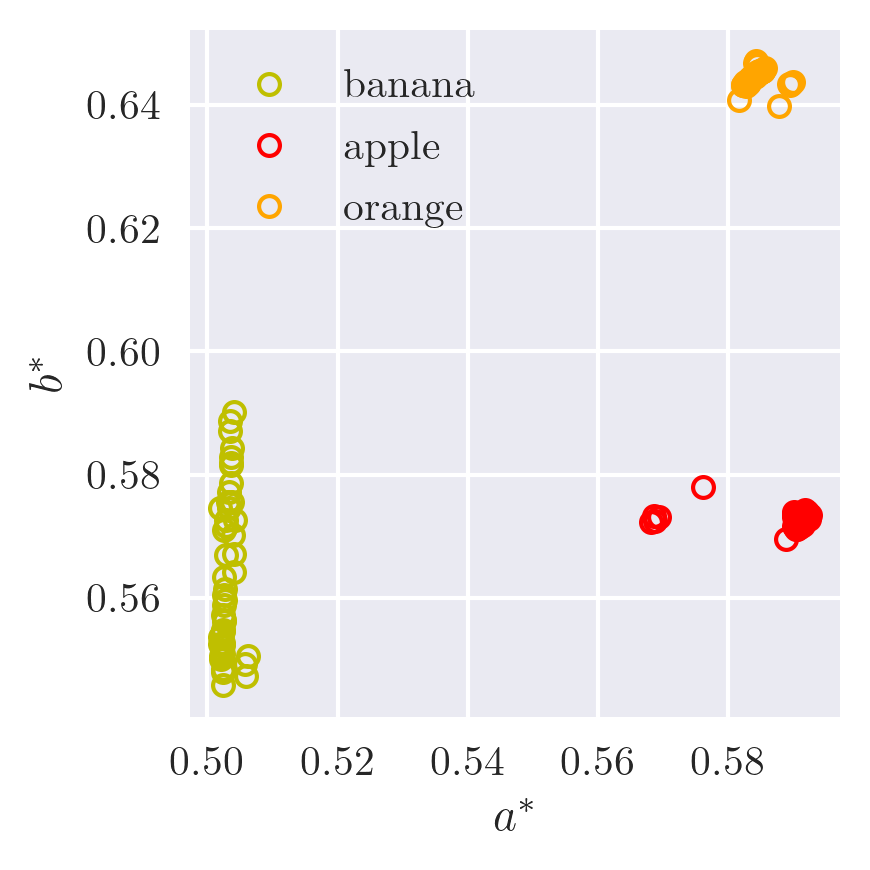
\includegraphics[width=\textwidth]{ab_space.png}
		\caption{$a^*$--$b^*$}
		\label{fig:ab-space}
	\end{subfigure}
	\begin{subfigure}[h!]{0.3\textwidth}
		\centering
		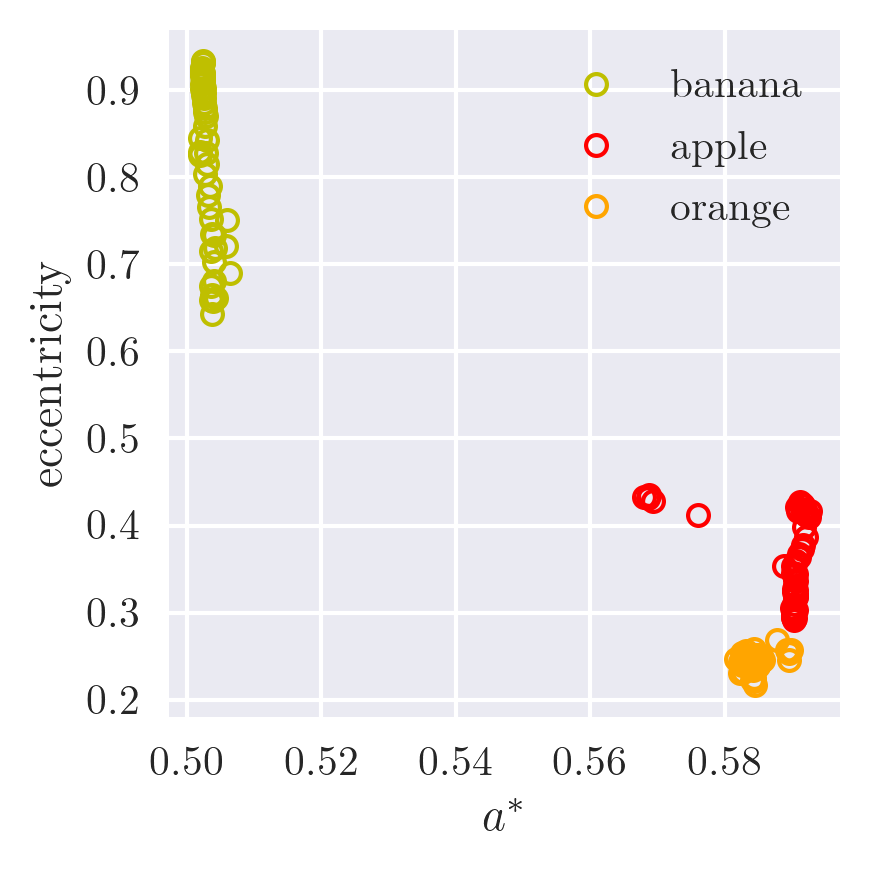
\includegraphics[width=\textwidth]{ae_space.png}
		\caption{$a^*$--$e$}
		\label{fig:ae-space}
	\end{subfigure}
	\begin{subfigure}[h!]{0.3\textwidth}
		\centering
		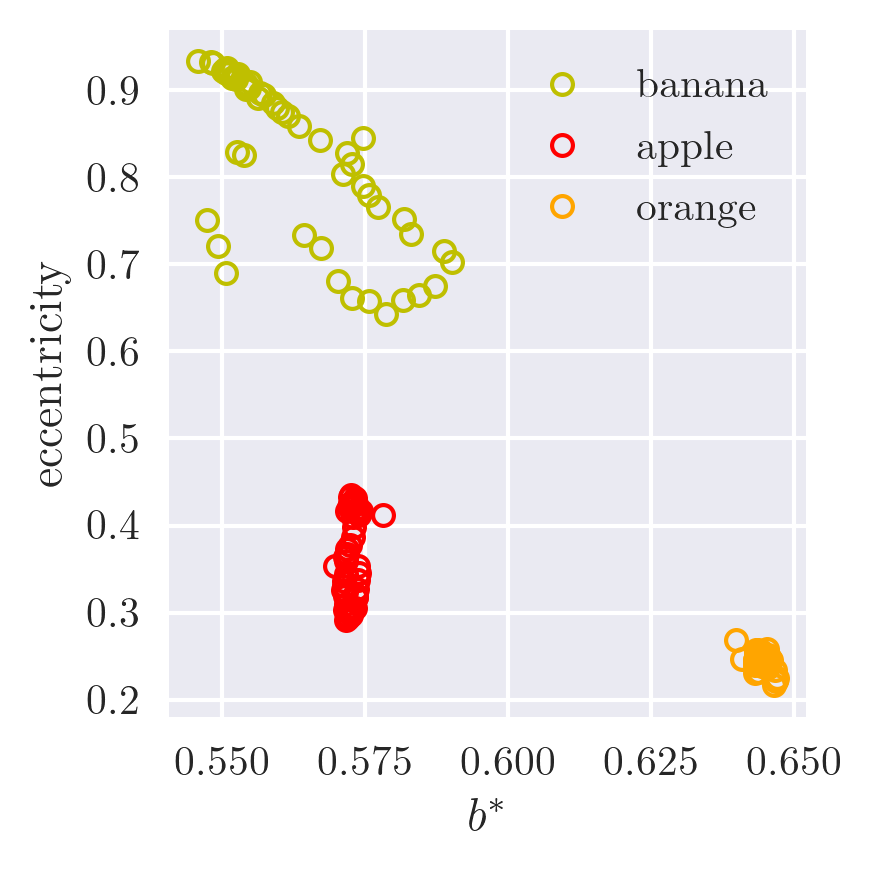
\includegraphics[width=\textwidth]{be_space.png}
		\caption{$b^*$--$e$}
		\label{fig:be-space}
	\end{subfigure}
	\caption{Feature space projections on different planes.}
	\label{fig:projections}
\end{figure}

\clearpage
\begin{table}[!htb]
	\centering
	\caption{Self-evaluation.}
	\begin{tabular}{||r|c||}
		\hline
		Technical correctness & 5 \\ \hline
		Quality of presentation & 5 \\ \hline
		Initiative & 0 \\ \hline
		\textbf{TOTAL} & \textbf{10} \\ \hline
	\end{tabular}
	\label{tab:self-eval}
\end{table}

\bibliographystyle{spp-bst}
\bibliography{biblio}

\end{document}